\documentclass[12pt]{article}
%DIF LATEXDIFF DIFFERENCE FILE



\usepackage{amsmath, mathtools}
\usepackage{amsfonts}
\usepackage{amssymb}
\usepackage{graphicx}
\usepackage{colortbl}
\usepackage{xr}
\usepackage{hyperref}
\usepackage{longtable}
\usepackage{xfrac}
\usepackage{tabularx}
\usepackage{float}
\usepackage{siunitx}
\usepackage{booktabs}
\usepackage{caption}
\usepackage{pdflscape}
\usepackage{afterpage}
\usepackage{tikz}
\usepackage[round]{natbib}

%\usepackage{refcheck}

\hypersetup{
    bookmarks=true,         % show bookmarks bar?
      colorlinks=true,       % false: boxed links; true: colored links
    linkcolor=red,          % color of internal links (change box color with linkbordercolor)
    citecolor=green,        % color of links to bibliography
    filecolor=magenta,      % color of file links
    urlcolor=cyan           % color of external links
}

%\input{../Comments}
%%% Common Parts

\newcommand{\progname}{ProgName} % PUT YOUR PROGRAM NAME HERE %Every program
                                % should have a name

\usepackage{hyperref}
    \hypersetup{colorlinks=true, linkcolor=blue, citecolor=blue, filecolor=blue,
                urlcolor=blue, unicode=false}
    \urlstyle{same}
                                


% For easy change of table widths
\newcommand{\colZwidth}{1.0\textwidth}
\newcommand{\colAwidth}{0.13\textwidth}
\newcommand{\colBwidth}{0.82\textwidth}
\newcommand{\colCwidth}{0.1\textwidth}
\newcommand{\colDwidth}{0.05\textwidth}
\newcommand{\colEwidth}{0.8\textwidth}
\newcommand{\colFwidth}{0.17\textwidth}
\newcommand{\colGwidth}{0.5\textwidth}
\newcommand{\colHwidth}{0.28\textwidth}

% Used so that cross-references have a meaningful prefix
\newcounter{defnum} %Definition Number
\newcommand{\dthedefnum}{GD\thedefnum}
\newcommand{\dref}[1]{GD\ref{#1}}
\newcounter{datadefnum} %Datadefinition Number
\newcommand{\ddthedatadefnum}{DD\thedatadefnum}
\newcommand{\ddref}[1]{DD\ref{#1}}
\newcounter{theorynum} %Theory Number
\newcommand{\tthetheorynum}{T\thetheorynum}
\newcommand{\tref}[1]{T\ref{#1}}
\newcounter{tablenum} %Table Number
\newcommand{\tbthetablenum}{T\thetablenum}
\newcommand{\tbref}[1]{TB\ref{#1}}
\newcounter{assumpnum} %Assumption Number
\newcommand{\atheassumpnum}{P\theassumpnum}
\newcommand{\aref}[1]{A\ref{#1}}
\newcounter{goalnum} %Goal Number
\newcommand{\gthegoalnum}{P\thegoalnum}
\newcommand{\gsref}[1]{GS\ref{#1}}
\newcounter{instnum} %Instance Number
\newcommand{\itheinstnum}{IM\theinstnum}
\newcommand{\iref}[1]{IM\ref{#1}}
\newcounter{reqnum} %Requirement Number
\newcommand{\rthereqnum}{P\thereqnum}
\newcommand{\rref}[1]{R\ref{#1}}
\newcounter{nfrnum} %NFR Number
\newcommand{\rthenfrnum}{NFR\thenfrnum}
\newcommand{\nfrref}[1]{NFR\ref{#1}}
\newcounter{lcfrnum} %Likelihood of change functional requirement number
\newcommand{\lthelcfrnum}{LC\thelcfrnum}
\newcommand{\lcfrref}[1]{LC\ref{#1}}
\newcounter{lcnum} %Likely change number
\newcommand{\lthelcnum}{LC\thelcnum}
\newcommand{\lcref}[1]{LC\ref{#1}}
\newcounter{ucnum} %Unlikely change number


\usepackage{fullpage}

\newcommand{\deftheory}[9][Not Applicable]
{
\newpage
\noindent \rule{\textwidth}{0.5mm}

\paragraph{RefName: } \textbf{#2} \phantomsection 
\label{#2}

\paragraph{Label:} #3

\noindent \rule{\textwidth}{0.5mm}

\paragraph{Equation:}

#4

\paragraph{Description:}

#5

\paragraph{Notes:}

#6

\paragraph{Source:}

#7

\paragraph{Ref.\ By:}

#8

\paragraph{Preconditions for \hyperref[#2]{#2}:}
\label{#2_precond}

#9

\paragraph{Derivation for \hyperref[#2]{#2}:}
\label{#2_deriv}

#1

\noindent \rule{\textwidth}{0.5mm}

}
%DIF PREAMBLE EXTENSION ADDED BY LATEXDIFF
%DIF UNDERLINE PREAMBLE %DIF PREAMBLE
\RequirePackage{color}\definecolor{RED}{rgb}{1,0,0}\definecolor{BLUE}{rgb}{0,0,1} %DIF PREAMBLE
\providecommand{\DIFaddtex}[1]{{\protect\color{blue}\uwave{#1}}} %DIF PREAMBLE
\providecommand{\DIFdeltex}[1]{{\protect\color{red}\sout{#1}}}                      %DIF PREAMBLE
%DIF SAFE PREAMBLE %DIF PREAMBLE
\providecommand{\DIFaddbegin}{} %DIF PREAMBLE
\providecommand{\DIFaddend}{} %DIF PREAMBLE
\providecommand{\DIFdelbegin}{} %DIF PREAMBLE
\providecommand{\DIFdelend}{} %DIF PREAMBLE
\providecommand{\DIFmodbegin}{} %DIF PREAMBLE
\providecommand{\DIFmodend}{} %DIF PREAMBLE
%DIF FLOATSAFE PREAMBLE %DIF PREAMBLE
\providecommand{\DIFaddFL}[1]{\DIFadd{#1}} %DIF PREAMBLE
\providecommand{\DIFdelFL}[1]{\DIFdel{#1}} %DIF PREAMBLE
\providecommand{\DIFaddbeginFL}{} %DIF PREAMBLE
\providecommand{\DIFaddendFL}{} %DIF PREAMBLE
\providecommand{\DIFdelbeginFL}{} %DIF PREAMBLE
\providecommand{\DIFdelendFL}{} %DIF PREAMBLE
%DIF HYPERREF PREAMBLE %DIF PREAMBLE
\providecommand{\DIFadd}[1]{\texorpdfstring{\DIFaddtex{#1}}{#1}} %DIF PREAMBLE
\providecommand{\DIFdel}[1]{\texorpdfstring{\DIFdeltex{#1}}{}} %DIF PREAMBLE
\newcommand{\DIFscaledelfig}{0.5}
%DIF HIGHLIGHTGRAPHICS PREAMBLE %DIF PREAMBLE
\RequirePackage{settobox} %DIF PREAMBLE
\RequirePackage{letltxmacro} %DIF PREAMBLE
\newsavebox{\DIFdelgraphicsbox} %DIF PREAMBLE
\newlength{\DIFdelgraphicswidth} %DIF PREAMBLE
\newlength{\DIFdelgraphicsheight} %DIF PREAMBLE
% store original definition of \includegraphics %DIF PREAMBLE
\LetLtxMacro{\DIFOincludegraphics}{\includegraphics} %DIF PREAMBLE
\newcommand{\DIFaddincludegraphics}[2][]{{\color{blue}\fbox{\DIFOincludegraphics[#1]{#2}}}} %DIF PREAMBLE
\newcommand{\DIFdelincludegraphics}[2][]{% %DIF PREAMBLE
\sbox{\DIFdelgraphicsbox}{\DIFOincludegraphics[#1]{#2}}% %DIF PREAMBLE
\settoboxwidth{\DIFdelgraphicswidth}{\DIFdelgraphicsbox} %DIF PREAMBLE
\settoboxtotalheight{\DIFdelgraphicsheight}{\DIFdelgraphicsbox} %DIF PREAMBLE
\scalebox{\DIFscaledelfig}{% %DIF PREAMBLE
\parbox[b]{\DIFdelgraphicswidth}{\usebox{\DIFdelgraphicsbox}\\[-\baselineskip] \rule{\DIFdelgraphicswidth}{0em}}\llap{\resizebox{\DIFdelgraphicswidth}{\DIFdelgraphicsheight}{% %DIF PREAMBLE
\setlength{\unitlength}{\DIFdelgraphicswidth}% %DIF PREAMBLE
\begin{picture}(1,1)% %DIF PREAMBLE
\thicklines\linethickness{2pt} %DIF PREAMBLE
{\color[rgb]{1,0,0}\put(0,0){\framebox(1,1){}}}% %DIF PREAMBLE
{\color[rgb]{1,0,0}\put(0,0){\line( 1,1){1}}}% %DIF PREAMBLE
{\color[rgb]{1,0,0}\put(0,1){\line(1,-1){1}}}% %DIF PREAMBLE
\end{picture}% %DIF PREAMBLE
}\hspace*{3pt}}} %DIF PREAMBLE
} %DIF PREAMBLE
\LetLtxMacro{\DIFOaddbegin}{\DIFaddbegin} %DIF PREAMBLE
\LetLtxMacro{\DIFOaddend}{\DIFaddend} %DIF PREAMBLE
\LetLtxMacro{\DIFOdelbegin}{\DIFdelbegin} %DIF PREAMBLE
\LetLtxMacro{\DIFOdelend}{\DIFdelend} %DIF PREAMBLE
\DeclareRobustCommand{\DIFaddbegin}{\DIFOaddbegin \let\includegraphics\DIFaddincludegraphics} %DIF PREAMBLE
\DeclareRobustCommand{\DIFaddend}{\DIFOaddend \let\includegraphics\DIFOincludegraphics} %DIF PREAMBLE
\DeclareRobustCommand{\DIFdelbegin}{\DIFOdelbegin \let\includegraphics\DIFdelincludegraphics} %DIF PREAMBLE
\DeclareRobustCommand{\DIFdelend}{\DIFOaddend \let\includegraphics\DIFOincludegraphics} %DIF PREAMBLE
\LetLtxMacro{\DIFOaddbeginFL}{\DIFaddbeginFL} %DIF PREAMBLE
\LetLtxMacro{\DIFOaddendFL}{\DIFaddendFL} %DIF PREAMBLE
\LetLtxMacro{\DIFOdelbeginFL}{\DIFdelbeginFL} %DIF PREAMBLE
\LetLtxMacro{\DIFOdelendFL}{\DIFdelendFL} %DIF PREAMBLE
\DeclareRobustCommand{\DIFaddbeginFL}{\DIFOaddbeginFL \let\includegraphics\DIFaddincludegraphics} %DIF PREAMBLE
\DeclareRobustCommand{\DIFaddendFL}{\DIFOaddendFL \let\includegraphics\DIFOincludegraphics} %DIF PREAMBLE
\DeclareRobustCommand{\DIFdelbeginFL}{\DIFOdelbeginFL \let\includegraphics\DIFdelincludegraphics} %DIF PREAMBLE
\DeclareRobustCommand{\DIFdelendFL}{\DIFOaddendFL \let\includegraphics\DIFOincludegraphics} %DIF PREAMBLE
%DIF END PREAMBLE EXTENSION ADDED BY LATEXDIFF

\begin{document}
\begin{table}[hp]
\caption{Revision History} \label{TblRevisionHistory}
\begin{tabularx}{\textwidth}{llX}
\toprule
\textbf{Date} & \textbf{Developer(s)} & \textbf{Change}\\
\midrule
Oct $1^{th}$ & All & Initial division of labour\\
Oct $3^{rd}$ & All & Rough draft complete\\
Oct $5^{th}$ & All & Revision and proof-reading \\
Jan $23^{rd}$ & Jeffrey Dang & Changed placement of terms and terminology \\
\DIFaddbeginFL \DIFaddFL{April $2^{nd}$ }& \DIFaddFL{Michael Ilao }& \DIFaddFL{Rev1 updated document from instructor feedback + peer reviews }\\
\bottomrule
\end{tabularx}
\end{table}
\newpage

\title{Software Requirements Specification for SE 4G06 \\ An AI-based Approach to Designing Board Games} 
\author{Team \#6, Board Gamers
\\ Ilao Michael, ilaom
\\ Bedi Hargun, bedih
\\ Dang Jeffrey, dangj12
\\ Ada Jonah, karaatan
\\ Mai Tianzheng, mait6}
\date{\today}

\maketitle

~\newpage

\pagenumbering{arabic}

\tableofcontents

~\newpage

\section{Reference Material}
\DIFdelbegin %DIFDELCMD < 

%DIFDELCMD < %%%
\DIFdelend \DIFaddbegin \subsection{\DIFadd{Abbreviations and Acronyms}}
\renewcommand{\arraystretch}{1.2}
\begin{tabular}{l l} 
  \toprule		
  \textbf{\DIFadd{symbol}} & \textbf{\DIFadd{description}}\\
  \midrule 
  \DIFadd{SRS }& \DIFadd{Software Requirements Specification}\\
  \DIFadd{AI }& \DIFadd{Artificial Intelligence }\\
  \DIFadd{A }& \DIFadd{Assumption }\\
  \DIFadd{LC }& \DIFadd{Likely Change}\\
  \DIFadd{FR }& \DIFadd{Functional Requirement }\\
  \DIFadd{NFR }& \DIFadd{Non Functional Requirement }\\
  \DIFadd{FSM }& \DIFadd{Finite State Machine }\\ 
  \DIFadd{TA }& \DIFadd{Teaching Assistant }\\
  \bottomrule
\end{tabular}\\
\DIFaddend \subsection{Terminology and  Definitions}
This section is expressed in words, not with equations.  It provides the meaning of the different words and phrases used in the domain of the problem.
The terminology is used to introduce concepts from the world outside of the
mathematical model  The terminology provides a real-world connection to give the
mathematical model meaning.

This subsection provides a list of terms that are used in the subsequent
sections and their meaning, with the purpose of reducing ambiguity and making it easier to correctly understand the requirements:

\begin{itemize}

\item \textbf{AI Agent}: Refers to the subsystem that has an AI model trained to play the game at hand acting as one of the players of the game.

\item \textbf{Game Engine}: Refers to the subsystem that is an abstract representation of the actual game as software.

\item \textbf{Data Visualization}: Refers to the subsystem that visualizes Game Engine and AI Agent logs.

\item \textbf{Game State}: Refers to the state of the game, which could include player attributes, player score, and game layout. All attributes and characteristics that change throughout a game simulation are stored here.

\item \textbf{Observation Space}: Refers to the state of the game that is observable to a Game Agent. (Not all information is available to the Game Agents and can vary from agent to agent)

\item \textbf{Action Space}: Refers to the set of moves an AI Agent can take in a particular Game Engine.

\item \textbf{Game Designer}: The game designer is the person who is creating the game by coming up with the rules and writing a scenario for the game. The game designer will be the end user of the system to balance the game and improve the design of the game.

\DIFaddbegin \item \textbf{\DIFadd{Finite State Machine}}\DIFadd{: A finite state machine is a computation model that can be used to simulate sequential logic by using state, actions and transition functions that decide how a given action and state will transition to a new state. \mbox{%DIFAUXCMD
\cite{brilliant_math}
}\hskip0pt%DIFAUXCMD
}

\DIFaddend \end{itemize}

\newpage

\section{Introduction}
\subsection{Purpose of Document}

The purpose of this document is to define the needed features and intended \DIFdelbegin \DIFdel{behaviors }\DIFdelend \DIFaddbegin \DIFadd{behaviours }\DIFaddend of using an AI-based approach to designing board games. Both the users and software developers use this document as an agreement to involve important information such as system specification, goals of implementation, project constraints, functional and non-functional requirements. This document \DIFdelbegin \DIFdel{help }\DIFdelend \DIFaddbegin \DIFadd{helps }\DIFaddend software developers understand what the game users need, minimize the cost of time and money, split work into multiple smaller pieces, and get project development started on the right path.

\subsection{Scope of Requirements} 

The scope of our project is to create an AI-based, game simulation engine that can help identify pitfalls in a game’s mechanics and imbalances in the game’s scoring system. Our intended users are game developers who wish to use our application to develop a robust game. The AI engine, Game Engine, and the simulator will work together to create output for a decision tree visualization tool that will help the game developers identify various paths of decisions that led to specific end states. 
\\We have initially limited our scope to only have our application work with 2 games\DIFdelbegin \DIFdel{- }\DIFdelend \DIFaddbegin \DIFadd{: }\DIFaddend Tic-Tac-Toe, and \DIFdelbegin \DIFdel{Bellow Intent’s Age Contrived game}\DIFdelend \DIFaddbegin \href{https://www.anagecontrived.com/}{\DIFadd{Bellow Intent’s Age Contrived game}}\DIFadd{, \mbox{%DIFAUXCMD
\cite{AnAgeContrived}}\hskip0pt%DIFAUXCMD
}\DIFaddend . As a secondary goal, we will work towards having our application be an open-source framework such that it is possible for any game developer to use our system.


\subsection{Characteristics of Intended Reader} \label{sec_IntendedReader}
The intended readers of this document are Dr. Spencer Smith, Christopher Schankula (TA), Dr. Sebastien Mosser, and Dr. Vladimir Reinharz. This document is thus intended for an audience that has \DIFdelbegin \DIFdel{at minimum a high-level }\DIFdelend \DIFaddbegin \DIFadd{a }\DIFaddend technical understanding of game development, artificial intelligence, game simulation, and interfacing between low-coupled systems. As a result, the reader is expected to know the basic terminologies either through their own research or from an \DIFdelbegin \DIFdel{undergraduate level }\DIFdelend \DIFaddbegin \DIFadd{undergraduate-level }\DIFaddend course in all of the fields specified. This document will also be used by the developers of this project (members of Group 6), therefore, it is also intended as a guide for all future documents and milestones during the development of this project.
\newpage
\subsection{Stakeholders}
\begin{table}[h!]
\caption{Stakeholders} \label{Stakeholders}
\begin{tabularx}{\textwidth}{p{5cm}p{5cm}p{1.5cm}}
\toprule
Bellows Intent & Publisher of The Game\DIFdelbeginFL \DIFdelFL{"An Age Contrived" }\DIFdelendFL \DIFaddbeginFL \DIFaddFL{, }\emph{\DIFaddFL{An Age Contrived}} \DIFaddendFL & Primary\\
\midrule
Chris Matthew & Principal Author \DIFdelbeginFL \DIFdelFL{of "An Age Contrived" }\DIFdelendFL \DIFaddbeginFL \DIFaddFL{and Designer of }\emph{\DIFaddFL{An Age Contrived}} \DIFaddendFL and The Game Designer & Primary\\
\midrule
Dr. Sebastien Mosser & Supervisor & Secondary\\
\midrule
Dr Vladimir Reinharz & Supervisor & Secondary\\
\midrule
\DIFaddbeginFL \DIFaddFL{Other Game Designers }& \DIFaddFL{Potential Users }& \DIFaddFL{Tertiary}\\
\midrule
\DIFaddendFL Group \# 6 & Developers & Tertiary\\
\midrule
Players & & Tertiary\\
\midrule
\DIFaddFL{Society }& & \DIFaddFL{Tertiary}\\
\bottomrule
\end{tabularx}
\end{table}

\noindent 

\subsection{Organization of Document}

This SRS document is intended to be read in the order that the document is presented. The main sections are – scope, general system description, specific system description, functional and non-functional requirements, likely and unlikely changes, and traceability matrices.

\DIFaddbegin \DIFadd{The template of this document follows the 4G06 SRS template provided by }\href{https://github.com/smiths/capTemplate/tree/main/docs/SRS}{\DIFadd{Dr. Smith}} \DIFadd{\mbox{%DIFAUXCMD
\cite{srs_template}}\hskip0pt%DIFAUXCMD
. Below are the changes to this template
}\begin{itemize}
    \item \textbf{\DIFadd{Table of Units}}\DIFadd{: Removed
    }\item \textbf{\DIFadd{Table of Symbols}}\DIFadd{: Removed
    }\item \textbf{\DIFadd{Mathematical Notation}}\DIFadd{: Removed
    }\item \textbf{\DIFadd{Terminology and Definitions}}\DIFadd{: Moved to Section 1
    }\item \textbf{\DIFadd{Stakeholders}}\DIFadd{: Added
    }\item \textbf{\DIFadd{Normal Operation and Undesired Event Handling}}\DIFadd{: Added
    }\item \textbf{\DIFadd{Solution Characteristics Specification}}\DIFadd{: Replaced by Assumptions and Required Behaviour Overview
    }\item \textbf{\DIFadd{Likely Changes}}\DIFadd{: Combined into Likelihood of Changes for Functional Requirements
    }\item \textbf{\DIFadd{Unlikely Changes}}\DIFadd{: Combined into Likelihood of Changes for Functional Requirements
    }\item \textbf{\DIFadd{Impact Analysis}}\DIFadd{: Added
    }\item \textbf{\DIFadd{Values of Constants}}\DIFadd{: Added
    }\item \textbf{\DIFadd{Development Plan}}\DIFadd{: Removed
    }\item \textbf{\DIFadd{Reflection}}\DIFadd{: Added
}


\end{itemize}


\DIFadd{A table of contents is explicitly stated on page 3 with a table of contents to prime the reader on what is available in the document.
}


\DIFaddend \section{General System Description}

This section provides general information about the system.  It identifies the
interfaces between the system and its environment, describes the user
characteristics and lists the system constraints.

\subsection{System Context}

\DIFdelbegin \DIFdel{Figure 1 }\DIFdelend \DIFaddbegin \subsubsection{\DIFadd{System Architecture}}
\DIFadd{Figure \ref{Fig_SystemContext} }\DIFaddend shows the system architecture and how the different agents and components interact with their main inputs and outputs. Exact information is abstracted away as the architecture should allow for \DIFdelbegin \DIFdel{"swappable" }\DIFdelend \DIFaddbegin \DIFadd{change and swap of }\DIFaddend modules. Meaning \DIFdelbegin \DIFdel{if }\DIFdelend \DIFaddbegin \DIFadd{that }\DIFaddend different Game Engines and different AI Agents can be interchanged and the functionality of the system will stay the same, with different outcomes and performance. In this system user input is not given and the AI Agents act as \DIFdelbegin \DIFdel{"users " }\DIFdelend \DIFaddbegin \DIFadd{users }\DIFaddend that interact with the Game Engine giving commands and receiving data to make those decisions. There are two outputs from the Game Engine, first the new game state from a given move and then a log of the actions and state. This log is then read by a data visualizer that the real end user can view.

\begin{figure}[h!]
\begin{center}
 \includegraphics[width=1.0\textwidth]{SystemArchitecture.png}
\caption{System Context}
\label{Fig_SystemContext} 
\end{center}
\end{figure}

\DIFaddbegin \subsubsection{\DIFadd{Game Engine Subsystem}}
\label{sec:Game_Engine_SubSystem}
\DIFaddend Inside the Game Engine, there will be \DIFdelbegin \DIFdel{a finite state machine }\DIFdelend \DIFaddbegin \DIFadd{an FSM }\DIFaddend that controls the main game loop. The \DIFdelbegin \DIFdel{finite state automata }\DIFdelend \DIFaddbegin \DIFadd{FSM }\DIFaddend will be comprised of variables $<Q, \sum, \delta, q_{0}, F>$
\begin{itemize}
    \item $Q$\DIFaddbegin \DIFadd{: }\DIFaddend The set of states, for many systems will be almost infinite as there are many different states the game can get to. Tic-Tac-Toe for example has only 23 unique winning states, while a game like chess has almost infinitely many\DIFdelbegin \DIFdel{,
    }\DIFdelend \DIFaddbegin \DIFadd{. 
    }\DIFaddend \item $\sum$\DIFaddbegin \DIFadd{: }\DIFaddend The alphabet is a list of all possible moves from one state to another.
    \item $\delta:(Q,\sum) \xrightarrow[]{} Q$\DIFaddbegin \DIFadd{: }\DIFaddend The transition function that will take the current state and a possible move and output the new updated state.
    \item $q_0$\DIFaddbegin \DIFadd{: }\DIFaddend The starting state, for Tic-Tac-Toe would be an empty board, for Monopoly would be an empty board, and all players with their starting money.
    \item \DIFdelbegin \DIFdel{$q_1$ The state after the game has began and will be looping through continuously until the game has concluded.
    }%DIFDELCMD < \item %%%
\item%DIFAUXCMD
\DIFdel{$q_2$ The final state afterwards the winning move is made in the game and concludes the system.
    }%DIFDELCMD < \item %%%
\item%DIFAUXCMD
\DIFdelend $F \subset Q$\DIFaddbegin \DIFadd{: }\DIFaddend The set of final states, this will be all the \DIFdelbegin \DIFdel{winning }\DIFdelend \DIFaddbegin \DIFadd{completed }\DIFaddend end game states for a player\DIFdelbegin \DIFdel{.
}\DIFdelend \DIFaddbegin \DIFadd{, in this case $q_2$
}\DIFaddend \end{itemize}
To simplify the set of states, only three will be used \DIFaddbegin \DIFadd{in this diagram}\DIFaddend : start, finish and in progress. These will be denoted as $q_0, q_1, q_2$ respectively. \DIFaddbegin \DIFadd{Although $q_1$ and $q_2$, can be comprised of many sub-states. 
}\DIFaddend 

\begin{figure}[h!]
\begin{center}
\DIFdelbeginFL %DIFDELCMD < \begin{tikzpicture}[scale=0.2]
%DIFDELCMD < \tikzstyle{every node}+=[inner sep=0pt]
%DIFDELCMD < \draw [black] (10.6,-25.4) circle (3);
%DIFDELCMD < \draw (10.6,-25.4) node {$q0$};
%DIFDELCMD < \draw [black] (33,-25.4) circle (3);
%DIFDELCMD < \draw (33,-25.4) node {$q_1$};
%DIFDELCMD < \draw [black] (67.1,-25.4) circle (3);
%DIFDELCMD < \draw (67.1,-25.4) node {$q_2$};
%DIFDELCMD < \draw [black] (67.1,-25.4) circle (2.4);
%DIFDELCMD < \draw [black] (13.6,-25.4) -- (30,-25.4);
%DIFDELCMD < \fill [black] (30,-25.4) -- (29.2,-24.9) -- (29.2,-25.9);
%DIFDELCMD < \draw (21.8,-25.9) node [below] {$Begin\mbox{ }game$};
%DIFDELCMD < \draw [black] (36,-25.4) -- (64.1,-25.4);
%DIFDELCMD < \fill [black] (64.1,-25.4) -- (63.3,-24.9) -- (63.3,-25.9);
%DIFDELCMD < \draw (50.05,-25.9) node [below] {$Winning\mbox{ }move\mbox{ }is\mbox{ }played$};
%DIFDELCMD < \draw [black] (32.183,-22.525) arc (223.59229:-64.40771:2.25);
%DIFDELCMD < \draw (41.44,-16.94) node [above] {$Non-winning\mbox{ }valid\mbox{ }move\mbox{ }is\mbox{ }played$};
%DIFDELCMD < \fill [black] (34.78,-23) -- (35.71,-22.81) -- (35.02,-22.09);
%DIFDELCMD < \end{tikzpicture}
%DIFDELCMD < %%%
\DIFdelendFL \DIFaddbeginFL 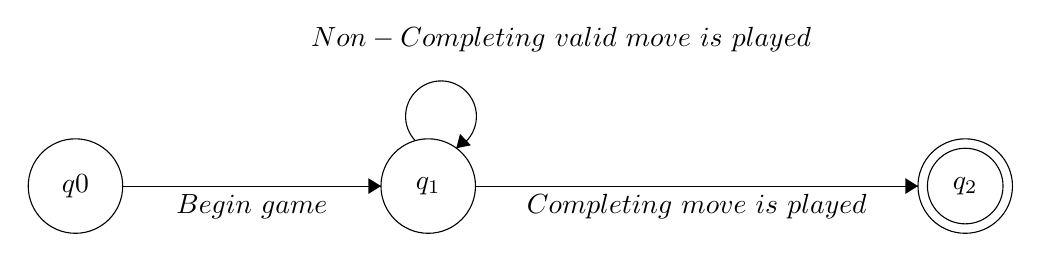
\begin{tikzpicture}[scale=0.2]
\tikzstyle{every node}+=[inner sep=0pt]
\draw [black] (10.6,-25.4) circle (3);
\draw (10.6,-25.4) node {$q0$};
\draw [black] (33,-25.4) circle (3);
\draw (33,-25.4) node {$q_1$};
\draw [black] (67.1,-25.4) circle (3);
\draw (67.1,-25.4) node {$q_2$};
\draw [black] (67.1,-25.4) circle (2.4);
\draw [black] (13.6,-25.4) -- (30,-25.4);
\fill [black] (30,-25.4) -- (29.2,-24.9) -- (29.2,-25.9);
\draw (21.8,-25.9) node [below] {$Begin\mbox{ }game$};
\draw [black] (36,-25.4) -- (64.1,-25.4);
\fill [black] (64.1,-25.4) -- (63.3,-24.9) -- (63.3,-25.9);
\draw (50.05,-25.9) node [below] {$Completing\mbox{ }move\mbox{ }is\mbox{ }played$};
\draw [black] (32.183,-22.525) arc (223.59229:-64.40771:2.25);
\draw (41.44,-16.94) node [above] {$Non-Completing\mbox{ }valid\mbox{ }move\mbox{ }is\mbox{ }played$};
\fill [black] (34.78,-23) -- (35.71,-22.81) -- (35.02,-22.09);
\end{tikzpicture}
\DIFaddendFL \caption{Finite State Machine for Game Loop}
\DIFaddbeginFL \label{Fig_FSM} 
\DIFaddendFL \end{center}
\end{figure}
The game will continue until a \DIFdelbegin \DIFdel{winning }\DIFdelend \DIFaddbegin \DIFadd{game completing }\DIFaddend move is played and loops after each \DIFdelbegin \DIFdel{non-winning }\DIFdelend \DIFaddbegin \DIFadd{non-completing }\DIFaddend move, and all non-valid moves are rejected. Based on the game non-valid moves could result in the game being forfeited and lost, for this simple example, the Game Engine will reject the AI Agent's move and wait for a valid \DIFdelbegin \DIFdel{one. 
}%DIFDELCMD < \\ 
%DIFDELCMD < %%%
\DIFdelend \DIFaddbegin \DIFadd{ones. 
}\DIFaddend 

\DIFaddbegin \DIFadd{Since our architecture will support multiple game engines, the FSM is generalized. As the FSM can be as simple as tic-tac-toe which will not have as many states as our complex game, }\emph{\DIFadd{An Age Contrived}}\DIFadd{. It is not feasible to fully describe either game in detail here as the diagram for the FSM will be too large too fit. As seen here \mbox{%DIFAUXCMD
\cite{erikras}}\hskip0pt%DIFAUXCMD
, a tic-tac-toe game has a possible 5,478 game states to track. The way $q_1$ will work is it will contain all possible states that the game can be in, in which it is not completed and the connections between each state are the game actions taken to travel between states. Now take this simpler version of tic-tac-toe in Figure \ref{Fig_TicTacToe} where a player needs to get 2 in a row. (Some final states are repeated, due to simplicity and easier to visualize). This simple game can be described as.
}\begin{itemize}
    \item \DIFadd{Q: - - -, X - -, - X -, O X -, etc... (All combinations of 1 X, 1 X and 1 O, and 2 X's and 1 O).
    }\item \DIFadd{$\sum$: L, M, R, where to play the next character: left, middle or right
    }\item \DIFadd{$\delta$: Transition function will take the state and action, and place an X or O, depending who's turn it is in that space.
    }\item \DIFadd{$q_0$ our initial state is - - -
    }\item \DIFadd{$F$: are all the states with 3 characters (X,X,0). For example XXO, OXX, etc...
}\end{itemize}
\begin{figure}[h!]
\begin{center}
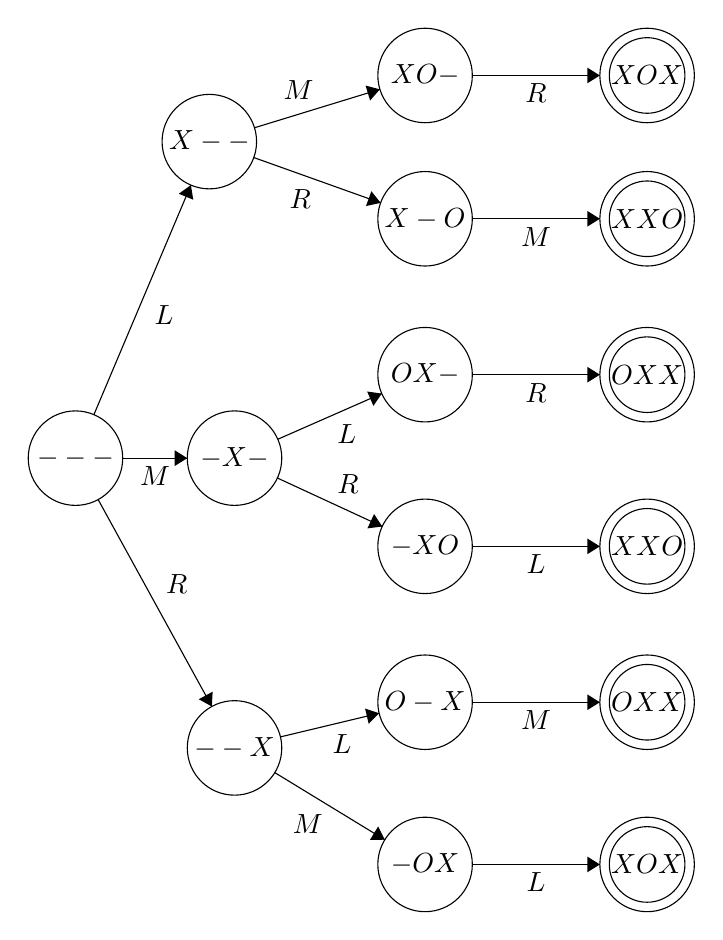
\begin{tikzpicture}[scale=0.2]
\tikzstyle{every node}+=[inner sep=0pt]
\draw [black] (5.4,-29.1) circle (3);
\draw (5.4,-29.1) node {$---$};
\draw [black] (13.9,-9) circle (3);
\draw (13.9,-9) node {$X--$};
\draw [black] (15.5,-29.1) circle (3);
\draw (15.5,-29.1) node {$-X-$};
\draw [black] (15.5,-47.5) circle (3);
\draw (15.5,-47.5) node {$--X$};
\draw [black] (27.6,-4.8) circle (3);
\draw (27.6,-4.8) node {$XO-$};
\draw [black] (27.6,-13.9) circle (3);
\draw (27.6,-13.9) node {$X-O$};
\draw [black] (27.6,-23.8) circle (3);
\draw (27.6,-23.8) node {$OX-$};
\draw [black] (27.6,-34.7) circle (3);
\draw (27.6,-34.7) node {$-XO$};
\draw [black] (27.6,-44.6) circle (3);
\draw (27.6,-44.6) node {$O-X$};
\draw [black] (27.6,-54.9) circle (3);
\draw (27.6,-54.9) node {$-OX$};
\draw [black] (41.7,-4.8) circle (3);
\draw (41.7,-4.8) node {$XOX$};
\draw [black] (41.7,-4.8) circle (2.4);
\draw [black] (41.7,-13.9) circle (3);
\draw (41.7,-13.9) node {$XXO$};
\draw [black] (41.7,-13.9) circle (2.4);
\draw [black] (41.7,-23.8) circle (3);
\draw (41.7,-23.8) node {$OXX$};
\draw [black] (41.7,-23.8) circle (2.4);
\draw [black] (41.7,-34.7) circle (3);
\draw (41.7,-34.7) node {$XXO$};
\draw [black] (41.7,-34.7) circle (2.4);
\draw [black] (41.7,-44.6) circle (3);
\draw (41.7,-44.6) node {$OXX$};
\draw [black] (41.7,-44.6) circle (2.4);
\draw [black] (41.7,-54.9) circle (3);
\draw (41.7,-54.9) node {$XOX$};
\draw [black] (41.7,-54.9) circle (2.4);
\draw [black] (8.4,-29.1) -- (12.5,-29.1);
\fill [black] (12.5,-29.1) -- (11.7,-28.6) -- (11.7,-29.6);
\draw (10.45,-29.6) node [below] {$M$};
\draw [black] (6.57,-26.34) -- (12.73,-11.76);
\fill [black] (12.73,-11.76) -- (11.96,-12.31) -- (12.88,-12.69);
\draw (10.39,-19.99) node [right] {$L$};
\draw [black] (6.84,-31.73) -- (14.06,-44.87);
\fill [black] (14.06,-44.87) -- (14.11,-43.93) -- (13.23,-44.41);
\draw (11.12,-37.11) node [right] {$R$};
\draw [black] (16.77,-8.12) -- (24.73,-5.68);
\fill [black] (24.73,-5.68) -- (23.82,-5.44) -- (24.11,-6.39);
\draw (19.57,-6.34) node [above] {$M$};
\draw [black] (30.6,-4.8) -- (38.7,-4.8);
\fill [black] (38.7,-4.8) -- (37.9,-4.3) -- (37.9,-5.3);
\draw (34.65,-5.3) node [below] {$R$};
\draw [black] (16.72,-10.01) -- (24.78,-12.89);
\fill [black] (24.78,-12.89) -- (24.19,-12.15) -- (23.85,-13.09);
\draw (19.68,-11.98) node [below] {$R$};
\draw [black] (30.6,-13.9) -- (38.7,-13.9);
\fill [black] (38.7,-13.9) -- (37.9,-13.4) -- (37.9,-14.4);
\draw (34.65,-14.4) node [below] {$M$};
\draw [black] (18.22,-30.36) -- (24.88,-33.44);
\fill [black] (24.88,-33.44) -- (24.36,-32.65) -- (23.94,-33.56);
\draw (22.7,-31.39) node [above] {$R$};
\draw [black] (18.25,-27.9) -- (24.85,-25);
\fill [black] (24.85,-25) -- (23.92,-24.87) -- (24.32,-25.78);
\draw (22.63,-26.96) node [below] {$L$};
\draw [black] (30.6,-23.8) -- (38.7,-23.8);
\fill [black] (38.7,-23.8) -- (37.9,-23.3) -- (37.9,-24.3);
\draw (34.65,-24.3) node [below] {$R$};
\draw [black] (30.6,-34.7) -- (38.7,-34.7);
\fill [black] (38.7,-34.7) -- (37.9,-34.2) -- (37.9,-35.2);
\draw (34.65,-35.2) node [below] {$L$};
\draw [black] (18.42,-46.8) -- (24.68,-45.3);
\fill [black] (24.68,-45.3) -- (23.79,-45) -- (24.02,-45.97);
\draw (22.32,-46.63) node [below] {$L$};
\draw [black] (18.06,-49.07) -- (25.04,-53.33);
\fill [black] (25.04,-53.33) -- (24.62,-52.49) -- (24.1,-53.34);
\draw (20.16,-51.7) node [below] {$M$};
\draw [black] (30.6,-44.6) -- (38.7,-44.6);
\fill [black] (38.7,-44.6) -- (37.9,-44.1) -- (37.9,-45.1);
\draw (34.65,-45.1) node [below] {$M$};
\draw [black] (30.6,-54.9) -- (38.7,-54.9);
\fill [black] (38.7,-54.9) -- (37.9,-54.4) -- (37.9,-55.4);
\draw (34.65,-55.4) node [below] {$L$};
\end{tikzpicture}
\caption{\DIFaddFL{Finite State Machine for Simple Tic Tac Toe}}
\label{Fig_TicTacToe} 
\end{center}
\end{figure}
\DIFadd{Even with this simple game the state space grows large, but it is an efficient way to track all possible states and how different actions take a player from state to state. Our AI will need to keep track of state and actions being taken as that is what our AI will learn from. Our AI will take each state as input and according to its decision making process, it will output an action, as seen in Figure \ref{Fig_FSM}.
}

\newpage
\subsubsection{\DIFadd{Responsibilities}}
\DIFaddend \textbf{User Responsibilities:}
\begin{itemize}
\item The Users will observe the data visualizer \DIFdelbegin \DIFdel{of game simulations}\DIFdelend \DIFaddbegin \DIFadd{that will display game simulation metrics}\DIFaddend . 
\end{itemize}


\textbf{System Responsibilities:}
\begin{itemize}
\item AI Agent: Receive input of a game state and output \DIFdelbegin \DIFdel{a decision}\DIFdelend \DIFaddbegin \DIFadd{an action}\DIFaddend . 
\item Available  Actions: List all available moves to the AI Agents (Not an entity itself and is a part of the Game Engine)
\item Game Engine: Receives \DIFdelbegin \DIFdel{inputs }\DIFdelend \DIFaddbegin \DIFadd{input }\DIFaddend of decisions made by the AI Agents and \DIFdelbegin \DIFdel{updates its }\DIFdelend \DIFaddbegin \DIFadd{update the }\DIFaddend game state accordingly. Outputs a log file of the \DIFaddbegin \DIFadd{game }\DIFaddend state and actions\DIFdelbegin \DIFdel{and the updated }\DIFdelend \DIFaddbegin \DIFadd{, and the output the new }\DIFaddend state back to the \DIFdelbegin \DIFdel{Game }\DIFdelend \DIFaddbegin \DIFadd{AI }\DIFaddend Agents.
\end{itemize}

\subsection{User Characteristics} \label{SecUserCharacteristics}
The intended users of the system will be AI research professors and game designers. These users will be observing the same output of the system, but analyzing it in a different way. The AI research professors will be using the output to analyze how different kinds of AI play a specific Game Engine. Meaning these users should have \DIFdelbegin \DIFdel{a deep }\DIFdelend \DIFaddbegin \DIFadd{an }\DIFaddend understanding of AI, Neural Networks, Machine Learning, and other AI topics. The game designers will be using the output to check for any \DIFdelbegin \DIFdel{"}\DIFdelend over-powered \DIFdelbegin \DIFdel{" }\DIFdelend strategies or game-breaking rules, these users should have a deep understanding of the game rules and mechanics (For the specific Game Engine in use). For all users of the system\DIFaddbegin \DIFadd{, they }\DIFaddend should have an understanding of statistics up to Stats 3Y03\DIFaddbegin \DIFadd{, }\DIFaddend to read and understand the data output.

\subsection{System Constraints}
The main constraint of the system is \DIFdelbegin \DIFdel{it }\DIFdelend \DIFaddbegin \DIFadd{the AI and Game Engine }\DIFaddend must be developed in Python\DIFaddbegin \DIFadd{, }\DIFaddend as AI libraries \DIFdelbegin \DIFdel{are }\DIFdelend \DIFaddbegin \DIFadd{in Python are the }\DIFaddend easiest to implement and highly supported\DIFdelbegin \DIFdel{, the Game Engine and all other components }\DIFdelend \DIFaddbegin \DIFadd{. The Game Engine }\DIFaddend must be implemented in Python for simple compatibility and integration. \DIFaddbegin \DIFadd{Potential libraries to be used for AI component of the system are }\href{https://gymnasium.farama.org/}{\DIFadd{Gymnasium}} \DIFadd{\mbox{%DIFAUXCMD
\cite{gymnasium_documentation}}\hskip0pt%DIFAUXCMD
, }\href{http://www.simple-ai.com/}{\DIFadd{Simple}} \DIFadd{\mbox{%DIFAUXCMD
\cite{simpleai} }\hskip0pt%DIFAUXCMD
or }\href{https://tianshou.readthedocs.io/en/master/}{\DIFadd{Tianshou}} \DIFadd{\mbox{%DIFAUXCMD
\cite{welcome_to_tianshou}}\hskip0pt%DIFAUXCMD
.
}\DIFaddend 

\DIFaddbegin \DIFadd{While Python must be used for the Game Engine and AI, the data visualizer can be developed in any language or library as coupling between the Data visualizer and the Game Engine is very low. Potential libraries for data visualizing are:
}\begin{itemize}
    \item \href{https://echarts.apache.org/en/index.html}{\DIFadd{Apache ECharts}} \DIFadd{\mbox{%DIFAUXCMD
\cite{apache_echarts}
    }\hskip0pt%DIFAUXCMD
}\item \href{https://plotly.com/python/}{\DIFadd{Plotly}} \DIFadd{\mbox{%DIFAUXCMD
\cite{plotly_python_graphing_library}
    }\hskip0pt%DIFAUXCMD
}\item \href{https://uber.github.io/react-vis/}{\DIFadd{react-vis}} \DIFadd{\mbox{%DIFAUXCMD
\cite{react-vis}
}\hskip0pt%DIFAUXCMD
}\end{itemize}

\DIFaddend \subsection{Normal Operation \& Undesired Event Handling}
The system will have a main loop where all the operations will take place after the initialization until the \DIFdelbegin \DIFdel{win }\DIFdelend \DIFaddbegin \DIFadd{game completion }\DIFaddend condition is reached, then the system will exit the loop and end the current game to provide data visualization. This initialization, main loop, and \DIFdelbegin \DIFdel{win }\DIFdelend \DIFaddbegin \DIFadd{game completion }\DIFaddend condition can be modeled \DIFdelbegin \DIFdel{and think as a finite state machine}\DIFdelend \DIFaddbegin \DIFadd{as an FSM}\DIFaddend . The process is explained in detail in Section \DIFdelbegin \DIFdel{2.1 }\DIFdelend \DIFaddbegin \DIFadd{\ref{sec:Game_Engine_SubSystem} }\DIFaddend and visualized in Figure \DIFdelbegin \DIFdel{2. In the event of an unexpected outcome, since the games to be simulated are extremely complex and each move changes the state }\DIFdelend \DIFaddbegin \DIFadd{\ref{Fig_FSM}.
}

\DIFadd{To minimize undesired outcomes, where a game reaches an illegal state, ex: tic-tac-toe, where O has more spaces than X at the end }\DIFaddend of the game\DIFdelbegin \DIFdel{significantly, }\DIFdelend \DIFaddbegin \DIFadd{, whenever an AI takes an illegal action that would proceed to this state, }\DIFaddend the simulation will start over instead of any error handling. This decision is justified by the fact that each simulation should take less than \DIFdelbegin \DIFdel{5 minutes }\DIFdelend \DIFaddbegin \DIFadd{The Speed Benchmark \ref{const:speed}, }\DIFaddend and no undesired event will have a harmful effect on the system. \DIFaddbegin \DIFadd{Also a large negative reward will be assigned to the AI, which in turn will make the AI less likely to take this move which causes an undesirable behaviour for the system. }\DIFaddend Thus, the cost of restarting \DIFaddbegin \DIFadd{the simulation }\DIFaddend is cheaper than any extensive undesired event handling since we would have to handle thousands of different scenarios if we were to decide to do undesired event handling rather than restarting that particular simulation. \DIFaddbegin \DIFadd{As well as training the AI to only take legal actions given a certain game state. 
}\DIFaddend 

\DIFdelbegin %DIFDELCMD < \newpage
%DIFDELCMD < %%%
\DIFdelend \DIFaddbegin \DIFadd{Actions are also only given to the AI if they are legal to take in that specific game state, this will minimize undesired outcomes as the action that needs to be taken to get to an illegal state will not be provided to the AI. For example for tic-tac-toe if an X is placed in the center, the O player will be given all the actions except the center tile to place its O. Referring back to Figure \ref{Fig_TicTacToe}, the only moves supplied after taking an action are the ones that haven't been taken. If L is taken first, the only moves available are M and R. Our system will be designed in a similar fashion where actions provided to the AI will be decided on the current state, in order to prevent illegal states.
}

\DIFadd{When an undesired event occurs and the simulation must restart, the output will be omitted from the game log, to ensure the data visualizer is only showing legal games that are played. Ensures all games visualized contain complete and un-corrupted data.
}

\DIFaddend \section{Specific System Description}

This section first presents the problem description, which gives a high-level
view of the problem to be solved.  This is followed by definitions and assumptions.

\subsection{Problem Description} \label{Sec_pd}

Designing a game is not an easy task. Especially, if the game is not \DIFdelbegin \DIFdel{a softwarethat }\DIFdelend \DIFaddbegin \DIFadd{software. That }\DIFaddend can be updated with \DIFdelbegin \DIFdel{correction and }\DIFdelend balancing patches later on\DIFaddbegin \DIFadd{, }\DIFaddend but a physical board game where an incorrect game design can result in significant financial and reputation costs \DIFaddbegin \DIFadd{as it is expensive or sometimes impossible to patch a physical board game}\DIFaddend . In complex games, there are multiple players, dozens of variables and actions that can be taken, and millions of possible scenarios that each decision and variable can cause. A good game should be a balanced one and \DIFdelbegin \DIFdel{should }\DIFdelend not contain any definitive way to win the game every single time to make it more competitive and fun. However, it is also \DIFdelbegin \DIFdel{humanly }\DIFdelend not possible to go through each scenario and balance all the variables to make sure there are no loopholes in the game. Our project is trying to create a process where game designers can see most of the scenarios and balance the game before even publishing by utilizing the power of computers.

\subsubsection{Goal Statements}

\noindent Given the inputs, the goal statements are:

\begin{itemize}

\item \textbf{Game Simulation}: The system must simulate good quality board games containing rules and strategies\DIFdelbegin \DIFdel{with no serious consequences of mistakes}\DIFdelend \DIFaddbegin \DIFadd{, that are not trivial ex: (Snakes and Ladders)}\DIFaddend .

\item \textbf{AI Learning}:
The system must implement artificial intelligent players to play thousands of games efficiently to detect patterns and learn winning strategies.   

\item \textbf{Complex Problem Solving}:
The AI game players of the system must be able to analyze complex decision paths. Each different AI game player should have a different decision-making process.  

\item \textbf{Quality Data}:
The system must output readable and correct data to track and save decisions, game states, and patterns throughout the simulations, as well as compare simulations against each other to find winning strategies.

\item \textbf{Data Visualization Analysis}:
The system must provide a variety of charts to visualize the data for users.

\DIFdelbegin %DIFDELCMD < \item %%%
\item%DIFAUXCMD
\textbf{\DIFdel{Live User Interface}}%DIFAUXCMD
\DIFdel{:
The system should have a live user interface where users can view the game states in real-time and the actions that AI game players are making.
}%DIFDELCMD < 

%DIFDELCMD < %%%
\DIFdelend \end{itemize}

\subsection{Assumptions} \label{sec_assumpt}

\begin{itemize}

\item[A\refstepcounter{assumpnum}\theassumpnum \label{A_Reward_Function}:]
  The game to be analyzed will have a clear reward function that AI Agent can optimize its learning towards. \DIFaddbegin \DIFadd{This reward function will be similar to the scoring/points system in the game.}\\ 
  \textbf{\DIFadd{Rationale}}\DIFadd{: The AI needs a reward to choose which moves are optimal in certain states.
  }\DIFaddend 

\item[A\refstepcounter{assumpnum}\theassumpnum \label{A_End_Condition}:]
  The game to be analyzed will have a clear win condition where the game ends.\\ 
  \textbf{Rationale}: It shouldn't be an open-ended, infinite game where the goal is to just increase your score\DIFaddbegin \DIFadd{, }\DIFaddend but rather there should be a specific condition(s) that players are playing towards to win and end the game. Otherwise, AI agents won't be able to find the optimal actions to win the game but rather keep outputting sub-optimal decisions which will have little to no value for game design improvements.

\item[A\refstepcounter{assumpnum}\theassumpnum \label{A_Representable}:]
  The game to be analyzed will have concrete rules that a computer can represent and enforce.\\
  \textbf{Rationale}: If the game cannot be simulated digitally, then AI Agent cannot be trained on the game and the system wouldn't be able to generate any meaningful data to aid the game design process.

\end{itemize}

\section{Required Behaviour Overview}
Our project consists of three main subsystems– Game Engine, AI Agent, and a data visualizer. These subsystems will work together to help game developers find imbalances in the game mechanics as well as find strategies that result in higher-than-expected winning percentages. 
\\\\
\textbf{AI Agent} – An AI model trained to play the game\DIFdelbegin \DIFdel{at hand }\DIFdelend \DIFaddbegin \DIFadd{, }\DIFaddend acting as one of the players \DIFdelbegin \DIFdel{of the game }\DIFdelend to give insights into the possible paths to be taken. It would analyze all possible paths that a player can take at any point in the game. It would take as input the game state information (current state and available moves for the player) and output the next move that the player will take. \DIFaddbegin \DIFadd{AI and all learning algorithms will be abstracted away by the libraries used so exact techniques and formulas for learning will not be required by the developers to implement.
}\DIFaddend \\
\textbf{Game Engine} – Abstract representation of the actual game as software. Contains all the game rules, observation space (state of the game), and action space (possible moves and commands that a player can choose from). It is also responsible for validating input from the AI Agent and outputting the game state with the moves available for the player. 
\\
\textbf{Data Visualizer} - Read the Game Engine and AI Agent log, and provide diverse graphic representations of data and information of moves to game state transitions. It will take the output from both the AI Agent and Game Engine to provide a way for the user to decipher imbalances in the game. \DIFaddbegin \DIFadd{The input and output of the system by the end-user (Game Designers) are only seen here as the data will be generated before hand and will be shown by the data visualizer, where the user can select different charts and graphs to visualize the data.
}\DIFaddend 


\section{Functional Requirements}

\subsection{AI Agent's Functional Requirements}
\noindent

\begin{minipage}{\textwidth}
\renewcommand*{\arraystretch}{1.5}
\begin{tabular}{| p{\colAwidth} | p{\colBwidth}|}
\hline
\rowcolor[gray]{0.9}
\bf FR\refstepcounter{reqnum}\thereqnum \DIFdelbegin %DIFDELCMD < \label{R_Input} %%%
\DIFdelend \DIFaddbegin \label{R_FR1} \DIFaddend & AI Agent \DIFdelbegin \DIFdel{should }\DIFdelend \DIFaddbegin \DIFadd{must }\DIFaddend take the state as input.\\ 
\hline
\bf Rationale & AI Agent will not store the state information. Rather it will get it from the Game Engine as an input.\\
\hline
\bf \DIFaddbegin \DIFadd{Verify }& \DIFadd{AI will output the same result given the same input after resetting the system.}\\
\hline
\bf \DIFaddend Priority& High\\
\hline
\end{tabular}
\end{minipage}\\

\begin{minipage}{\textwidth}
\renewcommand*{\arraystretch}{1.5}
\begin{tabular}{| p{\colAwidth} | p{\colBwidth}|}
\hline
\rowcolor[gray]{0.9}
\bf FR\refstepcounter{reqnum}\thereqnum \DIFdelbegin %DIFDELCMD < \label{R_Input} %%%
\DIFdelend \DIFaddbegin \label{R_FR2} \DIFaddend & AI Agent can be swapped with another AI Agent\DIFdelbegin \DIFdel{or a human player}\DIFdelend .\\ 
\hline
\bf Rationale & The project aims to provide a tool for all game designers to test their games. Every game will require a different AI model trained specifically on that game. Thus, AI \DIFdelbegin \DIFdel{Agent }\DIFdelend \DIFaddbegin \DIFadd{Agents }\DIFaddend needs to be modular enough to swap with other AI Agents. \\
\hline
\bf \DIFaddbegin \DIFadd{Verify }& \DIFadd{Change the AI and the system will still complete game simulations.}\\
\hline
\bf \DIFaddend Priority& Medium\\
\hline
\end{tabular}
\end{minipage}\\

\begin{minipage}{\textwidth}
\renewcommand*{\arraystretch}{1.5}
\begin{tabular}{| p{\colAwidth} | p{\colBwidth}|}
\hline
\rowcolor[gray]{0.9}
\bf FR\refstepcounter{reqnum}\thereqnum \DIFdelbegin %DIFDELCMD < \label{R_Input} %%%
\DIFdelend \DIFaddbegin \label{R_FR3} \DIFaddend & AI Agent \DIFdelbegin \DIFdel{should }\DIFdelend \DIFaddbegin \DIFadd{must }\DIFaddend be observable.\\ 
\hline
\bf Rationale & The decisions of the AI Agent should be recorded so that it can be reviewed by the game designer to guide the design of the board game.\\
\hline
\bf \DIFaddbegin \DIFadd{Verify }& \DIFadd{After each simulation an output of the game log will be generated.}\\
\hline
\bf \DIFaddend Priority& High\\
\hline
\end{tabular}
\end{minipage}\\

\begin{minipage}{\textwidth}
\renewcommand*{\arraystretch}{1.5}
\begin{tabular}{| p{\colAwidth} | p{\colBwidth}|}
\hline
\rowcolor[gray]{0.9}
\bf FR\refstepcounter{reqnum}\thereqnum \DIFdelbegin %DIFDELCMD < \label{R_Input} %%%
\DIFdelend \DIFaddbegin \label{R_FR4} \DIFaddend & AI Agent \DIFdelbegin \DIFdel{should }\DIFdelend \DIFaddbegin \DIFadd{must }\DIFaddend only output an action that is in the action space provided by the Game Engine.\\ 
\hline
\bf Rationale & By only selecting the actions in the action space provided by the Game Engine, errors will be reduced and the game can actually progress. \\
\hline
\bf \DIFaddbegin \DIFadd{Verify }& \DIFadd{Given a state check all illegal moves, these must be omitted from the action space}\\
\hline
\bf \DIFaddend Priority& High\\
\hline
\end{tabular}
\end{minipage}\\

\begin{minipage}{\textwidth}
\renewcommand*{\arraystretch}{1.5}
\begin{tabular}{| p{\colAwidth} | p{\colBwidth}|}
\hline
\rowcolor[gray]{0.9}
\bf FR\refstepcounter{reqnum}\thereqnum \DIFdelbegin %DIFDELCMD < \label{R_Input} %%%
\DIFdelend \DIFaddbegin \label{R_FR5} \DIFaddend & AI Agent shall not see the state information that a human player cannot see.\\ 
\hline
\bf Rationale & In multiplayer games, there will be information specific to the user (e.g. hidden cards) which the AI Agent should not see to have the same level of visibility as a human player would have. \\
\hline
\bf \DIFaddbegin \DIFadd{Verify }& \DIFadd{Check the game state each AI Agent observes and ensure they are only see hidden states that apply to them.}\\
\hline
\bf \DIFaddend Priority& High\\
\hline
\end{tabular}
\end{minipage}\\

\begin{minipage}{\textwidth}
\renewcommand*{\arraystretch}{1.5}
\begin{tabular}{| p{\colAwidth} | p{\colBwidth}|}
\hline
\rowcolor[gray]{0.9}
\bf FR\refstepcounter{reqnum}\thereqnum \DIFdelbegin %DIFDELCMD < \label{R_Input} %%%
\DIFdelend \DIFaddbegin \label{R_FR6} \DIFaddend & AI Agent shall always respond with an action.\\ 
\hline
\bf Rationale & Even if there is no optimal move, AI Agent should output an action so that the game can progress.\\
\hline
\bf \DIFaddbegin \DIFadd{Verify }& \DIFadd{Game simulation must complete even if the AI will lose.}\\
\hline
\bf \DIFaddend Priority& High\\
\hline
\end{tabular}
\end{minipage}\\

\subsection{Game Engine Functional Requirements}
\noindent

\begin{minipage}{\textwidth}
\renewcommand*{\arraystretch}{1.5}
\begin{tabular}{| p{\colAwidth} | p{\colBwidth}|}
\hline
\rowcolor[gray]{0.9}
\bf FR\refstepcounter{reqnum}\thereqnum \DIFdelbegin %DIFDELCMD < \label{R_Output} %%%
\DIFdelend \DIFaddbegin \label{R_FR7} \DIFaddend & The Game Engine must validate the input from the AI Agent\\ 
\hline
\bf Rationale& One of the core functionality of our system is the interaction between the AI Agent and the Game Engine. The Game Engine must be responsible for validating the input (state) from the AI engine, to ensure the action taken is a valid action. \\
\hline
\bf \DIFaddbegin \DIFadd{Verify }& \DIFadd{After receiving an action from the AI check if it is legal given the current game state.}\\
\hline
\bf \DIFaddend Priority& High\\
\hline
\end{tabular}
\end{minipage}\\

\begin{minipage}{\textwidth}
\renewcommand*{\arraystretch}{1.5}
\begin{tabular}{| p{\colAwidth} | p{\colBwidth}|}
\hline
\rowcolor[gray]{0.9}
\bf FR\refstepcounter{reqnum}\thereqnum \DIFdelbegin %DIFDELCMD < \label{R_Output} %%%
\DIFdelend \DIFaddbegin \label{R_FR8} \DIFaddend & The Game Engine must have an end/winning state to end the game.\\ 
\hline
\bf Rationale& A Game Engine's main role is to transition from the start state to the end state using the player's moves. The Game Engine must validate if a player(s) has reached the end state at any point of the gameplay.\\
\hline
\bf \DIFaddbegin \DIFadd{Verify }& \DIFadd{The game simulation must end.}\\
\hline
\bf \DIFaddend Priority& High\\
\hline
\end{tabular}
\end{minipage}\\

\begin{minipage}{\textwidth}
\renewcommand*{\arraystretch}{1.5}
\begin{tabular}{| p{\colAwidth} | p{\colBwidth}|}
\hline
\rowcolor[gray]{0.9}
\bf FR\refstepcounter{reqnum}\thereqnum \DIFdelbegin %DIFDELCMD < \label{R_Output} %%%
\DIFdelend \DIFaddbegin \label{R_FR9} \DIFaddend & The Game Engine must output the current state of the game, if not in the end state.\\ 
\hline
\bf Rationale& As the AI Agent will be using the Game Engine's output to perform different moves, it is essential for the Game Engine to provide the current state of the game in order for the AI to make appropriate decisions.\\
\hline
\bf \DIFaddbegin \DIFadd{Verify }& \DIFadd{Ensure after each action taken a new state is generated and provided to the AI}\\
\hline
\bf \DIFaddend Priority& High\\
\hline
\end{tabular}
\end{minipage}\\

\begin{minipage}{\textwidth}
\renewcommand*{\arraystretch}{1.5}
\begin{tabular}{| p{\colAwidth} | p{\colBwidth}|}
\hline
\rowcolor[gray]{0.9}
\bf FR\refstepcounter{reqnum}\thereqnum \DIFdelbegin %DIFDELCMD < \label{R_Output} %%%
\DIFdelend \DIFaddbegin \label{R_FR10} \DIFaddend & The Game Engine must follow all the playing and business rules of the game\\ 
\hline
\bf Rationale& It is necessary for the Game Engine to implement all the game rules such that it can validate moves and transition to the end state.\\
\hline
\bf \DIFaddbegin \DIFadd{Verify }& \DIFadd{Given a state and an action compare and ensure the new state that is generated is the same as described in the game rules. }\\
\hline
\bf \DIFaddend Priority& High\\
\hline
\end{tabular}
\end{minipage}\\

\begin{minipage}{\textwidth}
\renewcommand*{\arraystretch}{1.5}
\begin{tabular}{| p{\colAwidth} | p{\colBwidth}|}
\hline
\rowcolor[gray]{0.9}
\bf FR\refstepcounter{reqnum}\thereqnum \DIFdelbegin %DIFDELCMD < \label{R_Output} %%%
\DIFdelend \DIFaddbegin \label{R_FR11} \DIFaddend & The Game Engine must supply a list of game moves that an AI Agent can take.\\ 
\hline
\bf Rationale& It is necessary for the AI Agent to know what moves it can take. This move list does not ensure all moves are legal, only that they can be executed.\\
\hline
\bf \DIFaddbegin \DIFadd{Verify }& \DIFadd{Ensure AI is given a list of moves when it is there turn to take an action }\\
\hline
\bf \DIFaddend Priority& High\\
\hline
\end{tabular}
\end{minipage}\\


\subsection{Game Data Visualization Analysis Requirement}
\noindent

\begin{minipage}{\textwidth}
\renewcommand*{\arraystretch}{1.5}
\begin{tabular}{| p{\colAwidth} | p{\colBwidth}|}
\hline
\rowcolor[gray]{0.9}
\bf FR\refstepcounter{reqnum}\thereqnum \DIFdelbegin %DIFDELCMD < \label{R_Output} %%%
\DIFdelend \DIFaddbegin \label{R_FR12} \DIFaddend & The game system must generate a variety of data visualization charts\\ 
\hline
\bf Rationale &  The functionality of data visualization charts is to provide different graphic representations of data and information such as pie charts, bar graphs, and line charts to the users. It can efficiently show insights that may be missed in traditional reports and translates the data into a visual context that the users can understand easily.\\
\hline
\bf \DIFaddbegin \DIFadd{Verify }& \DIFadd{Generate more than Graph Number Benchmark \ref{const:graphnum} graphs and charts that represent different data points. }\\
\hline
\bf \DIFaddend Priority& High\\
\hline
\end{tabular}
\end{minipage}\\


\begin{minipage}{\textwidth}
\renewcommand*{\arraystretch}{1.5}
\begin{tabular}{| p{\colAwidth} | p{\colBwidth}|}
\hline
\rowcolor[gray]{0.9}
\bf FR\refstepcounter{reqnum}\thereqnum \DIFdelbegin %DIFDELCMD < \label{R_Output} %%%
\DIFdelend \DIFaddbegin \label{R_FR13} \DIFaddend & The game system must read data from the Game Engine and AI Agent logs. \\ 
\hline
\bf Rationale &  The functionality of reading data from the Game Engine and AI Agent allows the system to proceed with deeper data analysis.\\
\hline
\bf \DIFaddbegin \DIFadd{Verify }& \DIFadd{Ensure the data from the game engine matches what is visualized on the data visualizer. }\\
\hline
\bf \DIFaddend Priority& High\\
\hline
\end{tabular}
\end{minipage}\\

\begin{minipage}{\textwidth}
\renewcommand*{\arraystretch}{1.5}
\begin{tabular}{| p{\colAwidth} | p{\colBwidth}|}
\hline
\rowcolor[gray]{0.9}
\bf FR\refstepcounter{reqnum}\thereqnum \DIFdelbegin %DIFDELCMD < \label{R_Output} %%%
\DIFdelend \DIFaddbegin \label{R_FR14} \DIFaddend & The game system must allow users to select different data points  \\ 
\hline
\bf Rationale &  It is necessary for users to select a variety of data points such as win percentages of different first moves taken, game state changes in different decision-making processes, and actions having the highest win rates. \\
\hline
\bf \DIFaddbegin \DIFadd{Verify }& \DIFadd{Ensure data visualized changes between different data points }\\
\hline
\bf \DIFaddend Priority& High\\
\hline
\end{tabular}
\end{minipage}\\



\begin{minipage}{\textwidth}
\renewcommand*{\arraystretch}{1.5}
\begin{tabular}{| p{\colAwidth} | p{\colBwidth}|}
\hline
\rowcolor[gray]{0.9}
\bf FR\refstepcounter{reqnum}\thereqnum \DIFdelbegin %DIFDELCMD < \label{R_Output} %%%
\DIFdelend \DIFaddbegin \label{R_FR15} \DIFaddend & The game system \DIFaddbegin \DIFadd{must }\DIFaddend compare data between \DIFdelbegin \DIFdel{different Game Engine and AI Agent logs}\DIFdelend \DIFaddbegin \DIFadd{AI Agents}\DIFaddend .\\ 
\hline
\bf Rationale &  The functionality of data comparison evaluates and compares selected data points. For example, it can compare multiple AI players’ winning paths and output the most optimal option. \\
\hline
\bf \DIFaddbegin \DIFadd{Verify }& \DIFadd{Ensure the visualizer can view data from different AIs at once.}\\
\hline
\bf \DIFaddend Priority& Low\\
\hline
\end{tabular}
\end{minipage}\\


\newpage
\section{Nonfunctional Requirements}
This section will describe the non-functional requirements which will be the qualities the system has and why they are important and how they can be verified.

\subsection{Accuracy}
\begin{minipage}{\textwidth}
\renewcommand*{\arraystretch}{1.5}
\begin{tabular}{| p{\colAwidth} | p{\colBwidth}|}
\hline
\rowcolor[gray]{0.9}
\bf NFR\refstepcounter{nfrnum}\thenfrnum \label{NFR_Accuracy}: & The system, specifically the AI Agent \DIFdelbegin \DIFdel{should }\DIFdelend \DIFaddbegin \DIFadd{must }\DIFaddend get more and more accurate after each simulation in choosing winning moves. After \DIFdelbegin \DIFdel{(Learning Benchmark ) 1000 simulations }\DIFdelend \DIFaddbegin \DIFadd{reaching the Learning Benchmark \ref{const:learning}, }\DIFaddend an AI Agent \DIFdelbegin \DIFdel{should }\DIFdelend \DIFaddbegin \DIFadd{must }\DIFaddend be able to win against its previous version. \\ 
\hline
\bf Rationale & Since some of the AI \DIFdelbegin \DIFdel{Agent's }\DIFdelend \DIFaddbegin \DIFadd{Agents }\DIFaddend will be using reinforcement learning they must get more intelligent at playing the game after a duration of simulations. \\
\hline
\end{tabular}
\end{minipage}\\

\subsection{Usability}
\begin{minipage}{\textwidth}
\renewcommand*{\arraystretch}{1.5}
\begin{tabular}{| p{\colAwidth} | p{\colBwidth}|}
\hline
\rowcolor[gray]{0.9}
\bf NFR\refstepcounter{nfrnum}\thenfrnum \DIFdelbegin %DIFDELCMD < \label{NFR_Accuracy}%%%
\DIFdelend \DIFaddbegin \label{NFR_Usability}\DIFaddend : & The system \DIFdelbegin \DIFdel{should }\DIFdelend \DIFaddbegin \DIFadd{must }\DIFaddend be understood and navigable by the technical stakeholders (Dr. Mosser, Dr. Reinharz and Game Designers) after \DIFdelbegin \DIFdel{a (Understanding Benchmark ) 30-minute explanation }\DIFdelend \DIFaddbegin \DIFadd{an explanation length of the Understanding Benchmark \ref{const:understanding}, }\DIFaddend from the developers  \\ 
\hline
\bf Rationale & Usability of the system is not of high importance \DIFdelbegin \DIFdel{for }\DIFdelend \DIFaddbegin \DIFadd{to }\DIFaddend the general public. The main users will be AI Research Professors and Game Designers, these two users will only be interacting with one part of the system, that is the data visualizer. Users familiar with data visualization software \DIFdelbegin \DIFdel{should }\DIFdelend \DIFaddbegin \DIFadd{must }\DIFaddend have an easy time navigating and understanding the data \DIFaddbegin \DIFadd{if they have a Usability Benchmark \ref{const:usability} of data visualizing experience}\DIFaddend .\\
\hline
\end{tabular}
\end{minipage}\\

\subsection{Modularity}
\begin{minipage}{\textwidth}
\renewcommand*{\arraystretch}{1.5}
\begin{tabular}{| p{\colAwidth} | p{\colBwidth}|}
\hline
\rowcolor[gray]{0.9}
\bf NFR\refstepcounter{nfrnum}\thenfrnum \DIFdelbegin %DIFDELCMD < \label{NFR_Accuracy}%%%
\DIFdelend \DIFaddbegin \label{NFR_Modularity}\DIFaddend : & The system \DIFdelbegin \DIFdel{should }\DIFdelend \DIFaddbegin \DIFadd{must }\DIFaddend be modular enough to where additional AI Agents can be \DIFdelbegin \DIFdel{implemented in two days }\DIFdelend \DIFaddbegin \DIFadd{integrated in Modular Benchmark 1 \ref{const:modular1} }\DIFaddend of development time. A Game Engine can be \DIFdelbegin \DIFdel{implemented in 7 days }\DIFdelend \DIFaddbegin \DIFadd{integrated in Modular Benchmark 2 \ref{const:modular2} }\DIFaddend of development time.   \\ 
\hline
\bf Rationale & Modularity is a very important quality the system needs to have. All the components need to be easily swappable, that is AI Agents \DIFdelbegin \DIFdel{should }\DIFdelend \DIFaddbegin \DIFadd{must }\DIFaddend be able to be changed with other implementations of AI, with minimal effort and the structure \DIFdelbegin \DIFdel{should }\DIFdelend \DIFaddbegin \DIFadd{must }\DIFaddend support different Game Engines being integrated. \DIFaddbegin \DIFadd{These benchmarks are only for integration time within our system and not the actual development time it takes to create these components. }\DIFaddend \\
\hline
\end{tabular}
\end{minipage}\\

\subsection{Portability}
\begin{minipage}{\textwidth}
\renewcommand*{\arraystretch}{1.5}
\begin{tabular}{| p{\colAwidth} | p{\colBwidth}|}
\hline
\rowcolor[gray]{0.9}
\bf NFR\refstepcounter{nfrnum}\thenfrnum \DIFdelbegin %DIFDELCMD < \label{NFR_Accuracy}%%%
\DIFdelend \DIFaddbegin \label{NFR_Portability}\DIFaddend : & The system \DIFdelbegin \DIFdel{should }\DIFdelend \DIFaddbegin \DIFadd{must }\DIFaddend run on macOS Monterey and newer, Windows10 and newer, and on \DIFdelbegin \DIFdel{Aliance }\DIFdelend \DIFaddbegin \DIFadd{Alliance }\DIFaddend Canada's Computer Cluster. The simulation of the Game Engine with the AI Agent's must be able to run on each OS for them to be verified as working. \\ 
\hline
\bf Rationale & These operating systems will be used by the developers and the \DIFdelbegin \DIFdel{Aliance }\DIFdelend \DIFaddbegin \DIFadd{Alliance }\DIFaddend Canada's Computer Cluster will be used in case additional computing power is needed.\\
\hline
\end{tabular}
\end{minipage}\\

\subsection{Performance}
\begin{minipage}{\textwidth}
\renewcommand*{\arraystretch}{1.5}
\begin{tabular}{| p{\colAwidth} | p{\colBwidth}|}
\hline
\rowcolor[gray]{0.9}
\bf NFR\refstepcounter{nfrnum}\thenfrnum \DIFdelbegin %DIFDELCMD < \label{NFR_Accuracy}%%%
\DIFdelend \DIFaddbegin \label{NFR_Performance}\DIFaddend : & The system \DIFdelbegin \DIFdel{should }\DIFdelend \DIFaddbegin \DIFadd{must }\DIFaddend complete a single simulation in under \DIFdelbegin \DIFdel{(Speed Benchmark ) 5 minutes}\DIFdelend \DIFaddbegin \DIFadd{the Speed Benchmark \ref{const:speed}}\DIFaddend . \\ 
\hline
\bf Rationale & If a simulation is taking too long it will slow down the learning of the AI Agents as well as take up resources from the developers' computers.\\
\hline
\end{tabular}
\end{minipage}\\

\subsection{Extensibility}
\begin{minipage}{\textwidth}
\renewcommand*{\arraystretch}{1.5}
\begin{tabular}{| p{\colAwidth} | p{\colBwidth}|}
\hline
\rowcolor[gray]{0.9}
\bf NFR\refstepcounter{nfrnum}\thenfrnum \DIFdelbegin %DIFDELCMD < \label{NFR_Accuracy}%%%
\DIFdelend \DIFaddbegin \label{NFR_Extensibility}\DIFaddend : & The system \DIFdelbegin \DIFdel{should }\DIFdelend \DIFaddbegin \DIFadd{must }\DIFaddend be able to be extended to include additional rules and mechanics in \DIFdelbegin \DIFdel{2 days }\DIFdelend \DIFaddbegin \DIFadd{Extensible Benchmark \ref{const:extensible} }\DIFaddend of development time \DIFaddbegin \DIFadd{from a developer within the team}\DIFaddend . \\ 
\hline
\bf Rationale & With more complex games and games still in development rules and mechanics will be added iteratively rather than all at once.\\
\hline
\end{tabular}
\end{minipage}\\

\subsection{Look and Feel}
\begin{minipage}{\textwidth}
\renewcommand*{\arraystretch}{1.5}
\begin{tabular}{| p{\colAwidth} | p{\colBwidth}|}
\hline
\rowcolor[gray]{0.9}
\bf NFR\refstepcounter{nfrnum}\thenfrnum \DIFdelbegin %DIFDELCMD < \label{NFR_Accuracy}%%%
\DIFdelend \DIFaddbegin \label{NFR_LookFeel}\DIFaddend : & The system specifically the Data Visualizer \DIFdelbegin \DIFdel{should }\DIFdelend \DIFaddbegin \DIFadd{must }\DIFaddend clearly indicate data using different colours, lines and shapes. \DIFdelbegin \DIFdel{Should }\DIFdelend \DIFaddbegin \DIFadd{Must }\DIFaddend appeal to more than \DIFdelbegin \DIFdel{75\% (}\DIFdelend \DIFaddbegin \DIFadd{the }\DIFaddend Look Feel Benchmark \DIFdelbegin \DIFdel{) }\DIFdelend \DIFaddbegin \DIFadd{\ref{const:lookfeel} }\DIFaddend of game designers  \\ 
\hline
\bf Rationale & With a clear and clean look the data will be easier to visualize.\\
\hline
\end{tabular}
\end{minipage}\\
\subsection{Security}
N/A
\subsection{Cultural and Political}
N/A
\subsection{Legal}
N/A

\section{Phase-In Plan}
All requirements with \textit{High} priority must be implemented prior to the Revision 0 demonstration (February 6-17, 2023) as they represent the core functionality of our system.
\DIFaddbegin \begin{itemize}
    \item \DIFadd{FR1 \ref{R_FR1}
    }\item \DIFadd{FR3 \ref{R_FR3}
    }\item \DIFadd{FR4 \ref{R_FR4}
    }\item \DIFadd{FR5 \ref{R_FR5}
    }\item \DIFadd{FR6 \ref{R_FR6}
    }\item \DIFadd{FR7 \ref{R_FR7}
    }\item \DIFadd{FR8 \ref{R_FR8}
    }\item \DIFadd{FR9 \ref{R_FR9}
    }\item \DIFadd{FR10 \ref{R_FR10}
    }\item \DIFadd{FR11 \ref{R_FR11}
    }\item \DIFadd{FR12 \ref{R_FR12}
    }\item \DIFadd{FR13 \ref{R_FR13}
    }\item \DIFadd{FR14 \ref{R_FR14}
}\end{itemize}

\DIFaddend All requirements with \textit{Medium} priority will be implemented before the Revision 1 demonstration (March 20-31, 2023). 
\DIFaddbegin \begin{itemize}
    \item \DIFadd{FR2 \ref{R_FR2}
}\end{itemize}

\DIFaddend All requirements with \textit{Low} priority will be added after all \textit{High} and \textit{Medium} requirements are implemented, time permitting.
\DIFaddbegin 
\begin{itemize}
    \item \DIFadd{FR15 \ref{R_FR15}}
\end{itemize}

\DIFaddbegin \section{\DIFadd{Likelihood of Changes for Functional Requirements}}    
\DIFaddend \begin{table}[H]
\begin{tabular}{|l|p{0.20\textwidth}|p{0.34\textwidth}|p{0.20\textwidth}|l}
\cline{1-4}
\centering{\textbf{Requirement}} & \centering{\textbf{Likelihood of Change}} & \centering{\textbf{Rationale}}                                                                               & \centering{\textbf{Ways to Change}}                            &  \\ \cline{1-4}
\textbf{FR1}                                & Very Unlikely                                      & Core implementation aspect                                                                                            & N/A                                                                     &  \\ \cline{1-4}
\textbf{FR2}                                & Very Unlikely                                      & Core implementation aspect                                                                                            & N/A                                                                     &  \\ \cline{1-4}
\textbf{FR3}                                & Very Unlikely                                      & Core implementation aspect                                                                                            & N/A                                                                     &  \\ \cline{1-4}
\textbf{FR4}                                & Very Unlikely                                      & Must produce valid actions within the space or the system could loop indefinitely                                     & N/A                                                                     &  \\ \cline{1-4}
\textbf{FR5}                                & Very Unlikely                                      & AI Agent should not have an advantage over a human player                                                             & N/A                                                                     &  \\ \cline{1-4}
\textbf{FR6}                                & Very Unlikely                                      & Must produce an action or the system cannot continue function                                                         & N/A                                                                     &  \\ \cline{1-4}
\textbf{FR7}                                & Very Unlikely                                      & Core implementation aspect                                                                                            & N/A                                                                     &  \\ \cline{1-4}
\textbf{FR8}                                & Very Unlikely                                      & Core implementation aspect                                                                                            & N/A                                                                     &  \\ \cline{1-4}
\textbf{FR9}                                & Very Unlikely                                      & Important to visualize the state game for data analysis and allows for a human player to understand the state of game & N/A                                                                     &  \\ \cline{1-4}
\textbf{FR10}                               & Very Unlikely                                      & Core implementation aspect                                                                                            & N/A                                                                     &  \\ \cline{1-4}
\textbf{FR11}                               & Very Unlikely                                      & Allows for the AI Agent to generate a valid action to prevent invalid actions                                         & N/A                                                                     &  \\ \cline{1-4}
\textbf{FR12}                               & Unlikely                                           & May produce only a specific visualization data charts                                                                 & Produce only specific data visualization charts                         &  \\ \cline{1-4}
\textbf{FR13}                               & Very Unlikely                                      & Required for the stakeholder to understand the data                                                                   & N/A                                                                     &  \\ \cline{1-4}
\textbf{FR14}                               & Unlikely                                           & Subject to time constraints, is not required in the minimal viable product but highly valued for the stakeholder                                            & Requirement is removed and function is not implemented in final product &  \\ \cline{1-4}
\textbf{FR15}                               & Likely                                           & Subject to time constraints, is not required in the minimal viable product                                            & Requirement is removed and function is not implemented in final product &  \\ \cline{1-4}
\end{tabular}
\end{table}

\newpage
\section{Traceability Matrices and Graphs}
The table below shows the traceability matrix in how functional requirements depend on each other as well as depend on non-functional requirements and assumptions.
\begin{table}[h!]
\resizebox{17cm}{!} 
{
\begin{tabular}{|l|l|l|l|l|l|l|l|l|l|l|l|l|l|l|l|l|l|l|l|l|l|l|l|l|l|}
\hline
\textbf{ITEM} &
  \textbf{FR1} &
  \textbf{FR2} &
  \textbf{FR3} &
  \textbf{FR4} &
  \textbf{FR5} &
  \textbf{FR6} &
  \textbf{FR7} &
  \textbf{FR8} &
  \textbf{FR9} &
  \textbf{FR10} &
  \textbf{FR11} &
  \textbf{FR12} &
  \textbf{FR13} &
  \textbf{FR14} &
  \textbf{FR15} &
  \textbf{NFR1} &
  \textbf{NFR2} &
  \textbf{NFR3} &
  \textbf{NFR4} &
  \textbf{NFR5} &
  \textbf{NFR6} &
  \textbf{NFR7} &
  \textbf{A1} &
  \textbf{A2} &
  \textbf{A3} \\ \hline
\textbf{FR1}  &   &   &   &   &   &   &   &   & X &   &   &   &   &   &   & X &   & X &  & X & X &   &   &   &   \\ \hline
\textbf{FR2}  &   &   &   &   & X &   & X &   &   &   & X &   & X &   & X & X &   & X &  & X & X &   &   &   &   \\ \hline
\textbf{FR3}  &   &   &   &   &   &   &   &   &   &   &   &   & X &   & X &   &   &   &  &   &   &   &   &   &   \\ \hline
\textbf{FR4}  &   &   &   &   &   &   &   &   &   &   & X &   &   &   &   & X &   & X &  & X & X &   &   &   & X \\ \hline
\textbf{FR5}  &   & X &   &   &   &   &   &   &   &   &   &   &   &   &   &   &   &   &  &   &   &   &   &   &   \\ \hline
\textbf{FR6}  &   &   &   &   &   &   & X &   &   & X &   &   &   &   &   & X &   &   &  & X &   &   & X &   &   \\ \hline
\textbf{FR7}  &   & X &   &   &   & X &   &   &   &   &   &   &   &   &   &   &   &   &  &   &   &   &   &   & X \\ \hline
\textbf{FR8}  &   &   &   &   &   &   &   &   &   &   &   &   &   &   &   & X &   &   &  & X &   &   & X & X &   \\ \hline
\textbf{FR9}  & X &   &   &   &   &   &   &   &   &   &   &   &   &   &   &   &   &   &  & X &   &   &   &   &   \\ \hline
\textbf{FR10} &   &   &   &   &   & X &   &   &   &   &   &   &   &   &   &   &   &   &  &   &   &   &   &   & X \\ \hline
\textbf{FR11} &   & X &   & X &   &   &   &   &   &   &   &   &   &   &   & X &   &   &  &   &   &   &   &   &   \\ \hline
\textbf{FR12} &   &   &   &   &   &   &   &   &   &   &   &   &   &   &   &   & X &   &  &   &   & X &   &   &   \\ \hline
\textbf{FR13} &   & X & X &   &   &   &   &   &   &   &   &   &   &   &   &   &   &   &  &   &   &   &   &   &   \\ \hline
\textbf{FR14} &   &   &   &   &   &   &   &   &   &   &   &   &   &   &   &   & X &   &  &   &   & X &   &   &   \\ \hline
\textbf{FR15} &   & X & X &   &   &   &   &   &   &   &   &   &   &   &   &   & X &   &  &   &   & X &   &   &   \\ \hline
\textbf{NFR1} & X & X &   & X &   & X &   & X &   &   & X &   &   &   &   &   &   &   &  &   &   &   &   &   &   \\ \hline
\textbf{NFR2} &   &   & X &   &   &   &   &   &   &   &   & X &   & X & X &   &   &   &  &   &   &   &   &   &   \\ \hline
\textbf{NFR3} & X & X &   & X &   &   &   &   &   &   &   &   &   &   &   &   &   &   &  &   &   &   &   &   &   \\ \hline
\textbf{NFR4} &   &   &   &   &   &   &   &   &   &   &   &   &   &   &   &   &   &   &  &   &   &   &   &   &   \\ \hline
\textbf{NFR5} & X & X &   & X &   & X &   & X & X &   &   &   &   &   &   &   &   &   &  &   &   &   &   &   &   \\ \hline
\textbf{NFR6} & X & X &   & X &   &   &   &   &   &   &   &   &   &   &   &   &   &   &  &   &   &   &   &   &   \\ \hline
\textbf{NFR7} &   &   &   &   &   &   &   &   &   &   &   & X &   & X & X &   &   &   &  &   &   &   &   &   &   \\ \hline
\textbf{A1}   &   &   &   &   &   & X &   & X &   &   &   &   &   &   &   &   &   &   &  &   &   &   &   &   &   \\ \hline
\textbf{A2}   &   &   &   &   &   &   &   & X & X &   &   &   &   &   &   &   &   &   &  &   &   &   &   &   &   \\ \hline
\textbf{A3}   &   &   &   & X &   &   & X &   &   & X &   &   &   &   &   &   &   &   &  &   &   &   &   &   &   \\ \hline
\end{tabular}
}
\end{table}


\section{Impact Analysis}

This system will impact society as a stakeholder through the means of cultural factors as it is dealing with managing the quality of entertainment or specifically, the quality of board games. Completing this system will provide board game designers and game designers as a whole with a different and quicker means of balancing their turn-based games with AI. Being able to simulate many games in parallel to find unbalanced strategies in their games will allow them to produce these higher quality games for society to enjoy. In terms of health, safety, and other factors, this system will have a minimal impact. 

\DIFaddbegin \DIFadd{Cultural bias in this system will not be an issue as the data that the AI will learn from comes explicitly from the game engine which is a replication of the game rules and not from an outside source. There is no outside impact from society on the AI as it is bias-free and trains from a blank slate, we are not using any pre-trained models, but doing all the training from within our own system.
}

\DIFaddend \section{Values of Constants}
\DIFdelbegin %DIFDELCMD < \begin{itemize}
%DIFDELCMD < %%%
\DIFdelend \DIFaddbegin \begin{enumerate}
\DIFaddend \item \DIFaddbegin \label{const:graphnum}\DIFadd{Graph Benchmark: 5
}\item \label{const:learning}\DIFaddend Learning Benchmark: 1000 simulations
\item \DIFaddbegin \label{const:usability}\DIFadd{Usability Benchmark: 1 year
}\item \label{const:modular1}\DIFadd{Modular Benchmark 1: 2 days
}\item \label{const:modular2}\DIFadd{Modular Benchmark 2: 7 days
}\item \label{const:understanding}\DIFaddend Understanding Benchmark: 30 minutes
\item \DIFaddbegin \label{const:speed}\DIFaddend Speed Benchmark: 5 minutes \DIFaddbegin \DIFadd{on an average laptop with 8GB of RAM and at least i5 processor.
}\DIFaddend \item \DIFaddbegin \label{const:extensible}\DIFadd{Extensible Benchmark: 2 days
}\item \label{const:lookfeel}\DIFaddend Look and Feel Benchmark: 75\%
\DIFaddbegin \end{enumerate}
\DIFaddend 

\DIFdelbegin %DIFDELCMD < \end{itemize}
%DIFDELCMD < 

%DIFDELCMD < %%%
\DIFdelend \section{Reflection Appendix}
\subsection{Game mechanics and rules}
\\
Assigned Team Members: \textit{All}
\\
All team members will be required to thoroughly understand the game rules for all the games we will be working on. This knowledge and expertise will be acquired through playing the game, reading game rule books, and any online resources that explain the rules of the games.
\\\\
Every team member will be using all the discussed methods to gain \DIFdelbegin \DIFdel{the }\DIFdelend expertise in this domain as it is easy for everyone to understand the game rules by playing the game and then reading the game rule books to further enhance their knowledge.

\\
\subsection{AI Agent}
\\
Assigned Team Members: \textit{Jeffrey and Jonah}
\\
Learning how to develop and implement an AI Agent will require the knowledge and learning of specific AI APIs and libraries. The skills acquired from learning how these APIs and libraries work will allow the team to create feasible enough agents to generate viable moves for the Game Engine to accept. The team members assigned \DIFdelbegin \DIFdel{for }\DIFdelend \DIFaddbegin \DIFadd{to }\DIFaddend developing the AI Agents will begin with reinforcement learning libraries, Gym, PettingZoo, and SIMPLE, as a starting point to see if any viable AI Agents can be implemented with them and see if the team can further progress to other libraries. The team members were chosen for this topic for their previous experience in the machine learning course, COMPSCI 4ML3: Introduction to Machine Learning, and \DIFdelbegin \DIFdel{it }\DIFdelend should assist them in having to learn these libraries.
\\
Approaches to \DIFdelbegin \DIFdel{learn }\DIFdelend \DIFaddbegin \DIFadd{learning }\DIFaddend these libraries will involve dealing with tutorials, working with the starter code, and reading through the documentation.
\\\\
Jonah will use a combination of tutorials and documentation as he is able to understand better through tutorials and then he will be able to continue enforcing his knowledge further with the documentation given for the APIs and libraries.
\\\\
Jeffrey will begin by working on the starter code and continue will changing parameters in the starter code to see what output results as a consequence. Additionally, the use of the documentation will help change the starter code successfully. The reason for choosing this approach is because he particularly enjoys implementing first and then debugging towards the desired result afterward.
\subsection{Game Engine}
\\
Assigned Team Members: \textit{Michael and Hargun}
\\
Knowledge of Game Engine development and object-oriented programming is expected for this subsystem. The group members responsible for this subsystem will need to gain an understanding of how a Game Engine works and the level of abstraction it requires for it to be compatible with the other subsystems. The team members are also required to have experience with Python and have the thorough understanding principles of object-oriented programming. It is expected team members have a basic understanding of all libraries and frameworks that are used during the development of this subsystem. 
\\Knowledge and expertise will be gained through online tutorials, online articles, documentations of libraries/frameworks that are used, and through our supervisors.
\\\\Hargun will be using online tutorials and documentation to gain expertise in this domain area as it he finds it easier to learn from practical examples and then apply it to the desired problem.
\\\\Michael will be using online articles, documentation and our supervisors' expertise to gain knowledge in this domain area. Michael likes to research thoroughly before trying to solve a problem which is why it is beneficial for him to use these methods.


\subsection{Data Visualization Analysis}

Assigned Team Members: \textit{Tianzheng}
Data Visualization Analysis will require developers to understand users' expected data points, graphic representations, and what types of data need to compare. The group members are required to have sufficient knowledge of python data science libraries such as Matplotlib, Seaborn, NumPy, and pandas to create informative graphics and present accurate information to the users efficiently. 
\\\\
Tianzheng will be using online tutorials and documentation to gain expertise in data visualization and data analysis so as to find the most effective way to analyze the logs from the Game Engine and AI Agent. 
\newpage
\bibliographystyle{plainnat}
\bibliography{refs}
\DIFaddend 

\end{document}